\chapterhead{6}{Repairing a Model}{When a model is wrong, find out why and wrap it}\label{ch6}

A model that gives a wrong prediction is not useless. The job is to find \emph{why} it was wrong, then repair it. Often the model is fine for big questions and fails only for a small one. The repair is a better model for that small question, and the old model stays as it was, wrapped inside the new account.

\begin{center}
\sffamily\small\renewcommand{\arraystretch}{1.5}
\begin{tabular}{@{}p{3.4cm}p{3.7cm}p{3.7cm}@{}}
\toprule
\textbf{Model} & \textbf{What it keeps} & \textbf{What it drops}\\
\midrule
A $1:50$ model & rooms and big gaps & anything under 5~cm\\
A $1:10$ model & small gaps in one corner & the rest of the room\\
A repair & the old model and the fix & the claim it replaced\\
\bottomrule
\end{tabular}
\end{center}

\begin{tryit}{Repair it}
Find the question in chapter~5 with the smallest margin. Rebuild just that corner at $1:10$ and ask the question again.\par\medskip
\renewcommand{\arraystretch}{1.6}
\begin{tabular}{|l|c|c|c|c|}
\hline
\textbf{Scale} & \textbf{Model gap (cm)} & \textbf{Model thing (cm)} & \textbf{Model says} & \textbf{Real}\\ \hline
$1:50$ & & & & \\ \hline
$1:10$ & & & & \\ \hline
\end{tabular}
\end{tryit}

\begin{worked}{Practice numbers, not from a real room}
A chair is 59~cm wide. The real gap is 58~cm.\\
At $1:50$: gap $58\div50=1.16$, chair $59\div50=1.18$. A ruler marked in mm reads both as 1.2~cm, so the model says ``fits''. One mm on the model is 5~cm of room, too coarse.\\
At $1:10$: gap 5.8~cm, chair 5.9~cm. The chair is bigger. The model now says ``does not fit''. Real: it does not fit.
\end{worked}

\begin{center}
\begin{tikzpicture}
  \node[wrapcir,minimum size=3.2cm] (w) at (0,0) {};
  \node[bigcir,minimum size=1.8cm] (o) at (0,0) {}; \node[font=\sffamily\scriptsize,align=center] at (0,0) {old\\1:50};
  \node[cir] (n) at (4.6,0) {5.8}; \node[font=\sffamily\scriptsize] at (4.6,-0.9) {new, 1:10};
  \draw[moveA] (w) -- node[above,note] {repair} (n);
  \node[note,anchor=west,text width=3cm,align=left] at (5.6,0) {The old model stays inside the wrap. It still answers big questions.};
\end{tikzpicture}
\end{center}

\begin{multix}[hmm]\multixbot[hmm]\tcblower
The model said the chair fits, but it does not, so the model is broken. I will throw it in the bin and start again with nothing. Is that wise?
\end{multix}

\trust{We repeated the same question with the $1:10$ corner model and compared the answer with the real chair.}
{At $1:10$ one mm is only 1~cm of room, which is finer than the 1~cm margin, so the new answer is trustworthy for this question.}
{Other corners. We have only checked this one at $1:10$, and the new model says nothing about the rest of the room.}

\begin{keepbox}
We repaired a model for one question. \textbf{We kept} \wline[3.4cm] \textbf{and we set aside} \wline[3.4cm].
\end{keepbox}

\clearpage

\subhead{Spot the map that cheats}
All three maps show the same hallway, 6~m long, with a door that is 1~m wide. Two of them are drawn correctly. One is not.

\begin{center}
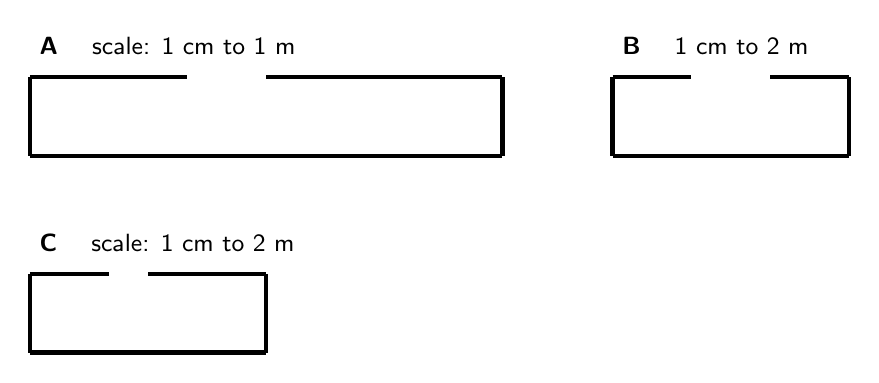
\begin{tikzpicture}[font=\sffamily\small]
  % A: 1 cm to 1 m, hallway 6 cm, door 1 cm
  \node[anchor=west] at (0,1.9) {\textbf{A} \quad scale: 1 cm to 1 m};
  \draw[line width=1.6pt] (0,0.5) -- (6,0.5); \draw[line width=1.6pt] (0,1.5) -- (2,1.5); \draw[line width=1.6pt] (3,1.5) -- (6,1.5);
  \draw[line width=1.6pt] (0,0.5) -- (0,1.5); \draw[line width=1.6pt] (6,0.5) -- (6,1.5);
  % B: 1 cm to 2 m, hallway 3 cm, door 1 cm (wrong)
  \node[anchor=west] at (7.4,1.9) {\textbf{B} \quad 1 cm to 2 m};
  \draw[line width=1.6pt] (7.4,0.5) -- (10.4,0.5); \draw[line width=1.6pt] (7.4,1.5) -- (8.4,1.5); \draw[line width=1.6pt] (9.4,1.5) -- (10.4,1.5);
  \draw[line width=1.6pt] (7.4,0.5) -- (7.4,1.5); \draw[line width=1.6pt] (10.4,0.5) -- (10.4,1.5);
  % C: 1 cm to 2 m, hallway 3 cm, door 0.5 cm
  \node[anchor=west] at (0,-0.6) {\textbf{C} \quad scale: 1 cm to 2 m};
  \draw[line width=1.6pt] (0,-2.0) -- (3,-2.0); \draw[line width=1.6pt] (0,-1.0) -- (1,-1.0); \draw[line width=1.6pt] (1.5,-1.0) -- (3,-1.0);
  \draw[line width=1.6pt] (0,-2.0) -- (0,-1.0); \draw[line width=1.6pt] (3,-2.0) -- (3,-1.0);
\end{tikzpicture}
\end{center}

Which map cheats? \wline[1.6cm] How wide would its door be in real life? \wline[1.6cm]~m\\[8pt]
Which map shows the door at its correct width with the smaller scale? \wline[1.6cm]

\clearpage

\begin{puzzle}{Reading precision}
At $1:50$, 1~mm on the model stands for \wline[1.6cm]~cm of room.
\end{puzzle}

\begin{puzzle}{Finer model}
At $1:10$, 1~mm on the model stands for \wline[1.6cm]~cm of room.
\end{puzzle}

\begin{puzzle}{Re-ask}
At $1:10$ the chair is 5.9~cm and the gap is 5.8~cm. Does the chair fit? \wline[2cm]
\end{puzzle}

\begin{puzzle}{Which first?}
A model said a 90~cm shelf fits a 95~cm gap, but the real gap is 88~cm. Name the first thing you would check. \wline[6cm]
\end{puzzle}

\begin{puzzle}{Bin or repair?}
Why is it better to repair a model than to throw it away? \wline[6cm]
\end{puzzle}

\clearpage

\begin{puzzle}{Pick the fix}
Choose a fix: (a) remeasure (b) a bigger scale for that corner (c) ask a different question. A $1:50$ model reads a 1~cm margin wrongly. \wline[1.6cm]
\end{puzzle}

\begin{puzzle}{Model or real?}
Write M for model and R for real thing.\\
(a) the $1:10$ corner \wline[1cm] \quad (b) the chair \wline[1cm] \quad (c) the old $1:50$ room \wline[1cm]
\end{puzzle}

\begin{puzzle}{Which question?}
Can the repaired corner model answer ``does the door open fully?'' \wline[2cm] What would it need? \wline[4cm]
\end{puzzle}

\begin{puzzle}{Unfair repair}
Ben made the corner at $1:10$ but measured the chair at $1:20$. Why does that mislead? \wline[6cm]
\end{puzzle}

\clearpage

\begin{puzzle}{Check backwards}
At $1:10$ the chair is 5.9~cm and the gap 5.8~cm. The real sizes are \wline[1.2cm]~cm and \wline[1.2cm]~cm. The difference is \wline[1.2cm]~cm.
\end{puzzle}

\begin{puzzle}{Wrap}
A student wrote ``The model was wrong.'' Wrap it with a better claim. \wline[6cm]
\end{puzzle}

\begin{puzzle}{A good habit}
Write one habit from this book that makes a model more trustworthy. \wline[6cm]
\end{puzzle}

\begin{puzzle}{Missing step}
A student built a model and said it was good without testing it once. What could go wrong? \wline[6cm]
\end{puzzle}

\clearpage

\begin{puzzle}{Draw the pair}
Draw the real chair and its model as two circles joined by a rule.
\begin{center}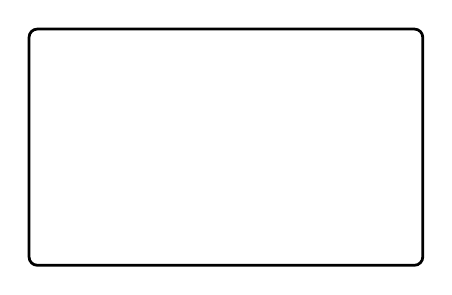
\begin{tikzpicture}\draw[line width=1pt,rounded corners=3pt] (0,0) rectangle (5,3); \end{tikzpicture}\end{center}
\end{puzzle}

\begin{puzzle}{Draw the repair}
Draw the $1:10$ corner with the old $1:50$ room still inside a dashed circle.
\begin{center}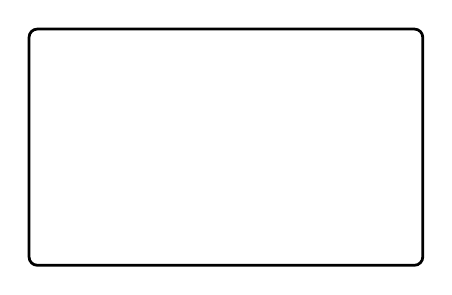
\begin{tikzpicture}\draw[line width=1pt,rounded corners=3pt] (0,0) rectangle (5,3); \end{tikzpicture}\end{center}
\end{puzzle}

\begin{puzzle}{Draw the wrap}
Draw a circle around ``the model was wrong'' and write the corrected claim outside it.
\begin{center}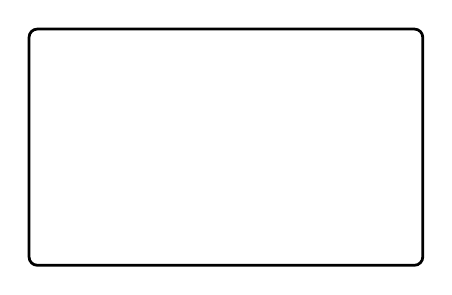
\begin{tikzpicture}\draw[line width=1pt,rounded corners=3pt] (0,0) rectangle (5,3); \end{tikzpicture}\end{center}
\end{puzzle}

\clearpage
\thispagestyle{fancy}\label{slop}
\subhead{Slop check}
Slop is hasty, gaudy work that forgot to take care. It can be made by a person or a machine, quickly or slowly. What matters is whether the work shows care for three things:
\begin{itemize}[leftmargin=1.6em]
\item \textbf{Salient:} Is the main point easy to see?
\item \textbf{Simple:} Is there anything that does nothing but get in the way?
\item \textbf{Relevant:} Does everything on the page help answer the question?
\end{itemize}

Here is a hasty poster about a hallway map. Study it, then decide what is wrong.

\begin{center}
\begin{tikzpicture}[scale=0.97]
  \fill[yellow!40,draw=purple!80!black,line width=3pt] (0,0) rectangle (11.4,7.6);
  \node[star,star points=12,fill=red!60,draw=blue,line width=2pt,minimum size=2.2cm,font=\bfseries\scriptsize,rotate=10,text=yellow] at (1.4,6.2) {WOW!!!};
  \node[font=\itshape\bfseries\Large,text=teal,rotate=-4] at (6.4,6.8) {mApS aRe MaGiC};
  \node[font=\ttfamily\tiny,text=orange] at (6.4,6.15) {(place maybe? who knows)};
  \foreach \x/\h/\c in {3/1.2/red,5.3/3.2/blue,7.6/5.0/green}{
    \fill[\c,draw=black] (\x,0.9) rectangle (\x+1.3,0.9+\h);
  }
  \node[font=\tiny,text=black,rotate=60] at (9.8,3) {number number number};
  \foreach \x/\y in {1.2/1.5,1.6/4.2,10.2/5.6,0.8/3}{\node[star,star points=5,fill=yellow,draw=red,minimum size=0.6cm] at (\x,\y) {};}
  \node[font=\tiny,text=lime!50!black] at (5.4,0.45) {map it!!!  best map ever!!!  wow  wow};
\end{tikzpicture}
\end{center}

\begin{slopbox}
\textbf{(a)} What is the poster's main point? Can you tell?\\[3pt]\rule{\linewidth}{0.5pt}\\[6pt]
\textbf{(b)} Name two things that are not simple, because they only distract.\\[3pt]\rule{\linewidth}{0.5pt}\\[6pt]
\textbf{(c)} Name two things that are missing, so the picture cannot be read.\\[3pt]\rule{\linewidth}{0.5pt}\\[6pt]
\textbf{(d)} Which part is not relevant to a hallway at all?\\[3pt]\rule{\linewidth}{0.5pt}
\end{slopbox}

\clearpage
\thispagestyle{fancy}
\subhead{Now you try}
On a separate sheet, redraw a clear map of a hallway: a hallway 12~m long and 2~m wide with doors at 2, 6 and 10~m, drawn at 1~cm to 1~m. Give it a title, add a scale bar, label the doors, use one or two calm colours, and delete everything that does not help. Check it against the three words: salient, simple, relevant.

\begin{center}
\begin{tikzpicture}
  \draw[ink!70,line width=1pt,rounded corners=3pt] (0,0) rectangle (11.4,1.0);
  \node[font=\sffamily\small,anchor=west] at (0.2,0.5) {Title:};
  \draw[ink!70,line width=1pt,rounded corners=3pt] (0,1.6) rectangle (11.4,9.6);
  \foreach \y in {2.6,3.6,...,8.6}{\draw[gray!30] (0,\y) -- (11.4,\y);}
  \foreach \x in {1,2,...,10}{\draw[gray!30] (\x,1.6) -- (\x,9.6);}
  \node[font=\sffamily\scriptsize,anchor=west] at (0.2,1.3) {Scale bar:};
\end{tikzpicture}
\end{center}

\clearpage
\thispagestyle{fancy}
\subhead{Build and test your own model}
Choose something real, such as a room, a desk, a path or a shelf. Write one question the model must answer, then build it, test it and say what it cannot do.\par\medskip
\renewcommand{\arraystretch}{1.7}
\begin{tabularx}{\linewidth}{|>{\sffamily\small\bfseries}p{3.0cm}|X|}
\hline
The real thing & \\ \hline
My question & \\ \hline
My scale & \\ \hline
What my model keeps & \\ \hline
What my model drops & \\ \hline
My prediction & \\ \hline
The real answer & \\ \hline
The gap, and the margin & \\ \hline
Questions it cannot answer & \\ \hline
\end{tabularx}
\par\bigskip\bigskip
\noindent Sketch the model and mark its scale.\par\medskip
\begin{tikzpicture}\draw[ink!70,line width=1pt,rounded corners=3pt] (0,0) rectangle (11.4,5.0);\end{tikzpicture}

\clearpage
\thispagestyle{fancy}
\subhead{What did we keep, across the whole course?}
Every book in Science built a model. For each book, write what the model kept and what it dropped. Book~1 is done for you. Use the hints in the second column.

\renewcommand{\arraystretch}{2.0}
\begin{center}\sffamily\scriptsize
\begin{tabularx}{\textwidth}{|>{\bfseries}p{2.6cm}|p{2.5cm}|X|X|}
\hline
\textbf{Book} & \textbf{Stood in for} & \textbf{What we kept} & \textbf{What we set aside} \\ \hline
1 The Ruler Is Never Exact & a length by a reading & the number and its error & the true length \\ \hline
2 A Fair Test & a whole by a trial & & \\ \hline
3 Shadows That Tell Time & a time by a shadow & & \\ \hline
4 Things That Push Back & a force by an arrow & & \\ \hline
5 Where the Water Goes & water by a count & & \\ \hline
6 Mixed Up and Sorted Out & a mixture by weights & & \\ \hline
7 Sorting the Living & a group by a key & & \\ \hline
8 Where the Energy Goes & energy by a height & & \\ \hline
9 Small Models, Big Things & a thing by a model & & \\ \hline
\end{tabularx}
\end{center}

\begin{multix}[wow]\multixbot[wow]\tcblower
Every model in this book was a stand-in. A stand-in is allowed to drop things, as long as you say which and test it against the real thing. Whenever you meet a map, a chart or a diagram, you will know to ask what it kept, what it dropped and which questions it was never built for.
\end{multix}

\clearpage
\thispagestyle{fancy}
\subhead{Write a model report}
\begin{tcolorbox}[enhanced,colback=white,colframe=ink!60,boxrule=1pt,arc=2mm,left=8pt,right=8pt,top=5pt,bottom=5pt]
\sffamily\small
\begin{enumerate}[leftmargin=1.6em,itemsep=0.2em]
\item \textbf{What I looked at.}
\item \textbf{What I changed, measured and kept the same.}
\item \textbf{My readings.} All of them.
\item \textbf{My answer.} With the gap named.
\item \textbf{What I kept and what it hides.}
\end{enumerate}
\end{tcolorbox}
\vspace{4pt}
Pick one model from this book and write a report on it. Use the lines below.\par\medskip
\foreach \i in {1,...,12}{\rule{\linewidth}{0.4pt}\\[18pt]}
\clearpage

\thispagestyle{fancy}
\subhead{Tests to try}
Pick one and design it with the habits from this book: change one thing, keep the rest the same, repeat, and test the model against the real thing.
\begin{enumerate}[leftmargin=1.6em,itemsep=0.5em]
\item Does a 1:20 model give smaller gaps than a 1:50 model?
\item Which is easier to follow, a map or a route diagram, for a stranger?
\item How closely can a model of your desk predict where a book will fit?
\item How much detail can a 1 cm to 5 m map of your street keep?
\item How wide must a gap be before a 1:50 model is safe?
\item Can a model of a shoebox predict how many fit on a shelf?
\end{enumerate}
\medskip
Write the test you pick:\par\medskip
\foreach \i in {1,...,6}{\rule{\linewidth}{0.4pt}\\[16pt]}
Change: \wline[3cm] Measure: \wline[3cm] Keep the same: \wline[3cm]
\clearpage

\thispagestyle{fancy}
\subhead{A week of models}
Each day, notice one model, such as a map, a chart or a toy, and say what it keeps and drops.\par\medskip
\renewcommand{\arraystretch}{3.2}
\begin{tabularx}{\linewidth}{|>{\sffamily\small\bfseries}p{1.8cm}|X|X|}
\hline
Day & The model & What it drops \\ \hline
Mon & & \\ \hline
Tue & & \\ \hline
Wed & & \\ \hline
Thu & & \\ \hline
Fri & & \\ \hline
Sat & & \\ \hline
Sun & & \\ \hline
\end{tabularx}
\clearpage

\thispagestyle{fancy}
\subhead{Questions I still have}
Write what you still wonder about models. Then pick one and think how to test it.\par\medskip
\foreach \i in {1,...,16}{\rule{\linewidth}{0.4pt}\\[16pt]}
